\documentclass{article}
\usepackage{graphicx}
\usepackage[margin=1.5cm]{geometry}
\usepackage{amsmath}

\begin{document}

\title{Thursday Reading Assessment: Unit 9, Torque and Angular Momentum}
\author{Prof. Jordan C. Hanson}

\maketitle

\section{Memory Bank}

\begin{itemize}
\item $\tau = r F \sin\theta$ ... Definition of torque.
\item Torque is the angular version of force.  It is the result of a force $F$, separated from a pivot by a distance $r$, that rotates the system about the pivot.  The angle between the force $F$ and the distance $r$ is $\theta$.
\item For sytems in \textit{static equilibrium}, the net force is zero, and the net torque is zero.
\item $\tau = I \alpha$ ... $I$ is the moment of inertia, and $\alpha$ is the angular acceleration.
\item $I = mr^2$ ... For a particle of mass $m$ rotating about a point from a radius $r$, $I$ is the moment of inertia.
\end{itemize}

\begin{figure}[ht]
\centering
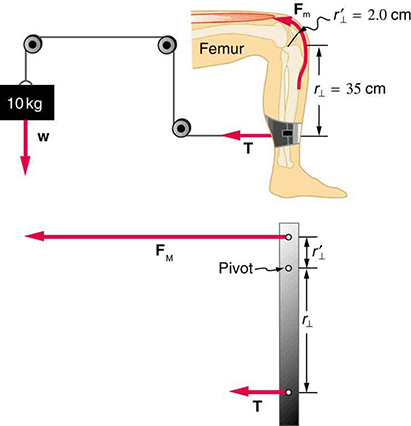
\includegraphics[width=0.25\textwidth]{figures/muscle1.jpeg}
\caption{\label{fig:torque} A person lifts a weight with their leg via an exercise machine.}
\end{figure}

\section{Torque}

\begin{enumerate}
\item A device for exercising the upper leg muscle is shown in Figure \ref{fig:torque}, together with a schematic representation of an equivalent lever system. Calculate the force exerted by the upper leg muscle to lift the mass at a constant speed. \\ \vspace{2cm}
\item Show using the following steps that $\tau = I \alpha$.
\begin{itemize}
\item Start with the definition of torque: $\tau = r F \sin\theta$, and assume $\theta = 90$ degrees.
\item Use Newton's 2nd law to substitute for the net force $F$.
\item Use $a = r\alpha$, the relationship between tangential acceleration $a$ and angular acceleration $\alpha$, to eliminate $a$.
\item Define $I = mr^2$, and substitute it into the current expression.
\item Do you see that $\tau = I \alpha$?
\end{itemize}
\end{enumerate}
\end{document}
